% !TEX root = main.tex

\section{Symbolic execution of binary code}

Challenges (e.g., ~\cite{BITBLAZE-ICISS08}):
\begin{enumerate}
\item Complexity of the instruction sets
\item Lack of a higher-level semantics (functions/CFG, types, buffers)
\item Obfuscation/dynamic code generation
\end{enumerate}

Symbolic techniques may work on the source code or on the binary code. However, it is not uncommon that both the former and the latter work by reasoning on an intermediate representation of the original code. For instance, ~\cite{KLEE-OSDI08} interprets the LLVM bytecode generated by compiling the source code, while~\cite{ANGR-SP16} reasons on the VEX IR that has been obtained by lifting the binary code.

\begin{figure}[h!]
  \centering
  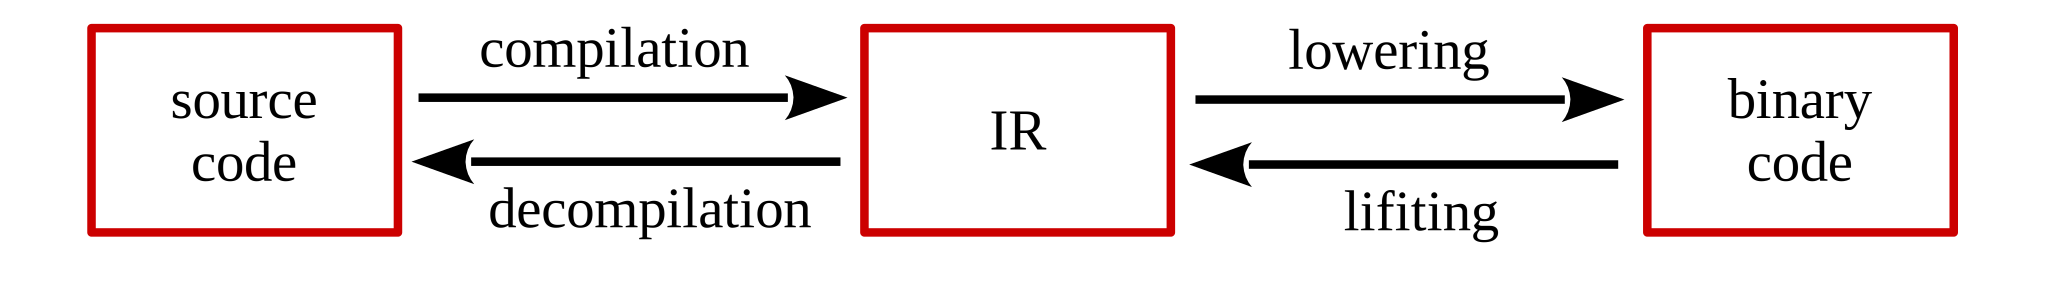
\includegraphics[width=.7\columnwidth]{images/compiler} 
\end{figure}